%%%%%%%%%%%%%%%%%%%%%%%%%%%%
%%%%%%%%%%%%%%%%%%%%%%%%%%%%
\section{Robustness} \label{sec:robustness}

As discussed in Section~\ref{sec:Motivation}, support values are a popular way to validate a focal tree. We present here the most popular ones. 

\begin{itemize}
 \item Confidence values based on resampling
 \item Assessments of other sources of error
\end{itemize}

%%%%%%%%%%%%%%%%%%%%%%%%%%%%
\subsection{Support Values} \label{sec:confidence-values}

%%%%%%%%%%%%%%%%%%%%%%%%%%%%
\subsubsection{Bootstrap} \label{sec:bootstrap}

Bootstrap values~\cite{Felsenstein1985} are probably the most popular and easiest to understand support values. Bootstrap involves resampling from one's molecular data with to create fictional datasets, called \emph{bootstrap replicates}, of the same size. Specifically, the molecular data is typically organized as a multiple sequence alignment (MSA) of $s$ species $\times$ $n$ characters. Since most models assume indenpendent characters, we generate a replicate by sampling $n$ characters, with replacement, from the original MSA and do this $B$ times. Note that in each replicate, some characters are sampled more than once and some left out entirely. The $B$ replicates are used to estimate a forest of $B$ bootstrap trees (one per replicate). Finally the bootstrap value ($BP$) of a branch of the original tree is its frequency of occurence in the forest. The process is illustrated in Figure~\ref{fig:bootstrap}. 

\begin{figure}
  \begin{center}
	\begin{tabular}{>{\centering\arraybackslash}m{4cm}cc}
	  \textbf{MSA} & & \textbf{Inferred Tree} \\
	  %% Original data
	  & \\
	  \multicolumn{3}{c}{Original Data}\\
	  $
	  \begin{array}{|c|cccc|}
	    \hline
	    \textbf{A} & \noir{A} & \gris{C} & \gray{T} & \grey{T} \\
	    \textbf{B} & \noir{G} & \gris{G} & \gray{A} & \grey{T} \\
	    \textbf{C} & \noir{G} & \gris{G} & \gray{C} & \grey{C} \\
	    \hline
	  \end{array}
	  $
	  &
	  $\longrightarrow$
	  &
	  \begin{minipage}[c]{0.25\linewidth}
	    \begin{center}
	      
\includegraphics[width=0.6\linewidth]{Figs/TrueOne3.pdf}
	    \end{center}
	  \end{minipage} 
	  \\
	  %% Replicate 1
	  & \\
	  \multicolumn{3}{c}{Bootstrap Replicate \#1}\\
	  $
	  \begin{array}{|c|cccc|}
	    \hline
	    \textbf{A} & \noir{A} & \gris{C} & \gray{T} & \gris{C} \\
	    \textbf{B} & \noir{G} & \gris{G} & \gray{A} & \gris{G} \\
	    \textbf{C} & \noir{G} & \gris{G} & \gray{C} & \gris{G} \\
	    \hline
	  \end{array}
	  $
	  &
	  $\longrightarrow$
	  &
	  \begin{minipage}[c]{0.25\linewidth}
	    \begin{center}
	      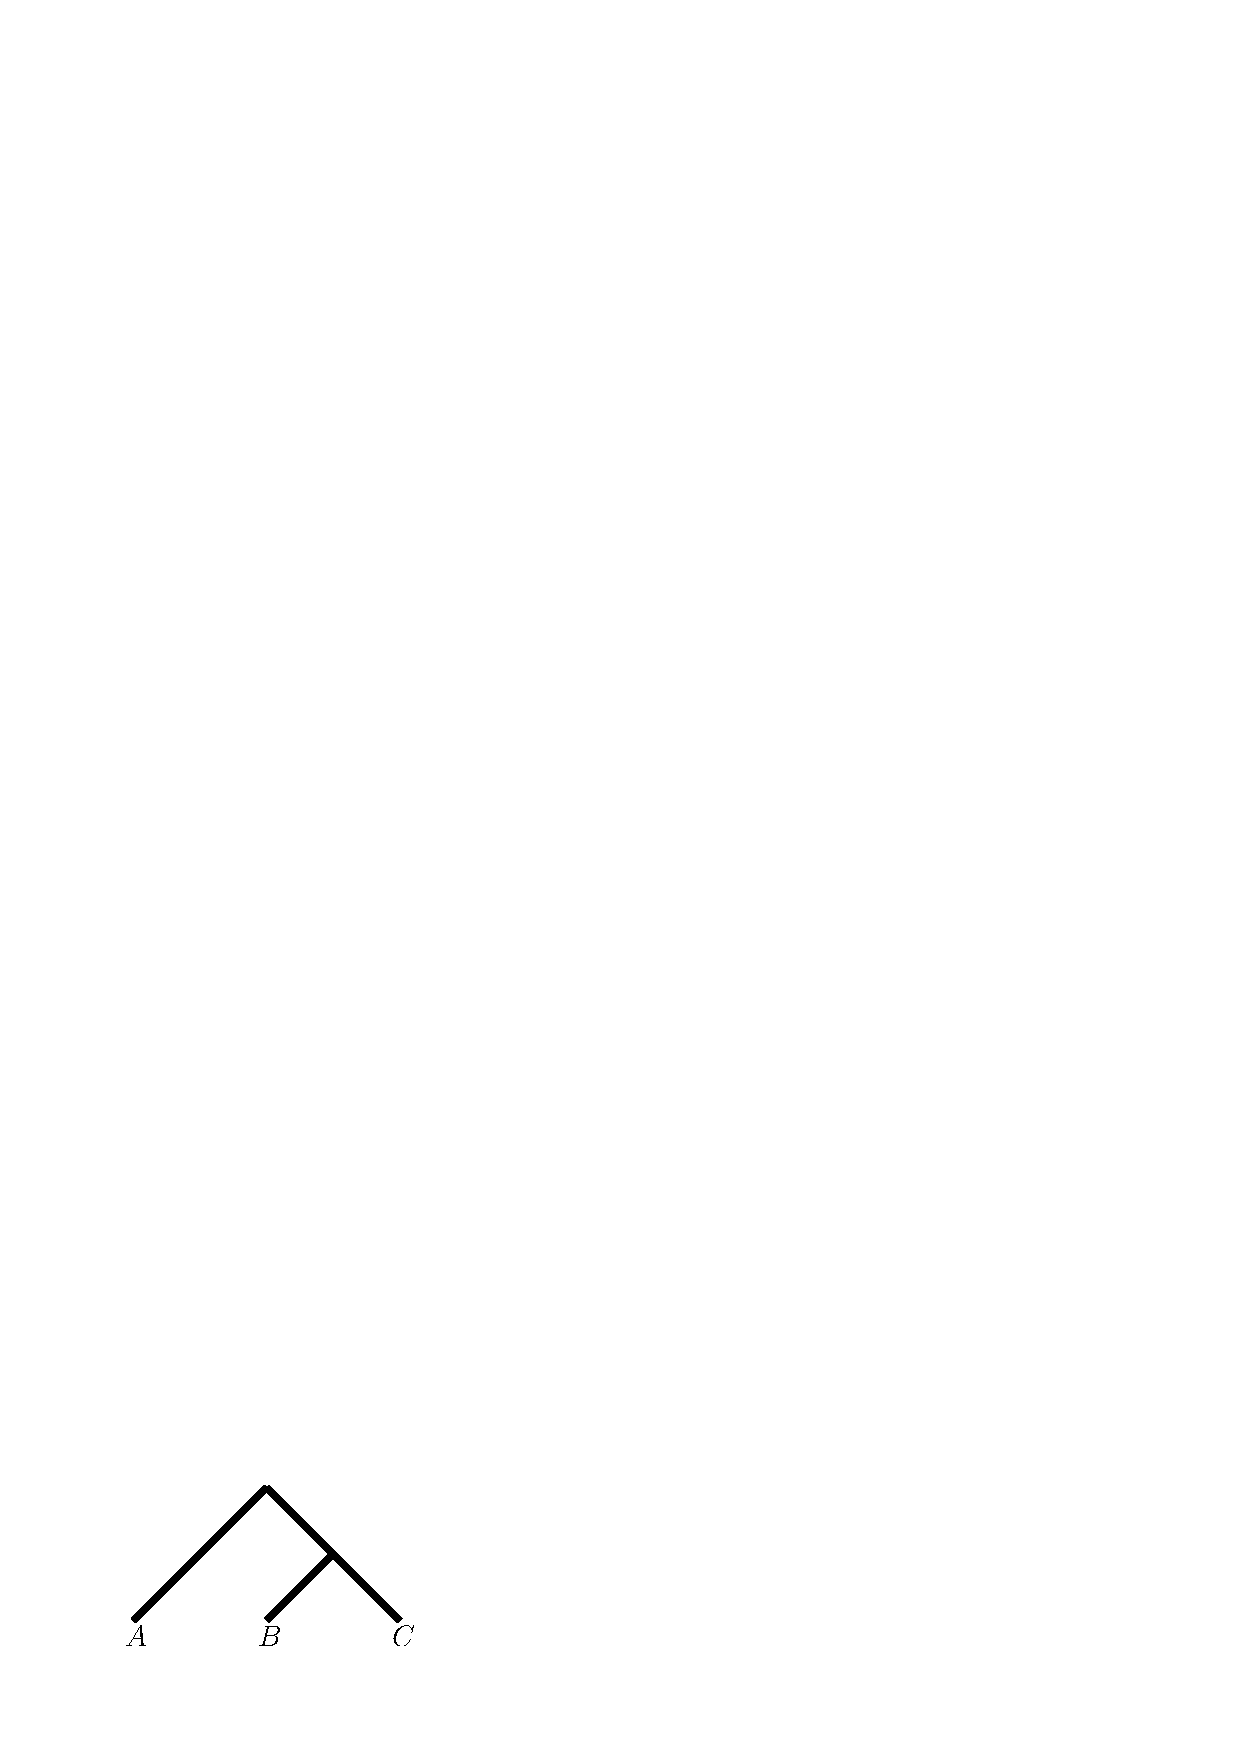
\includegraphics[width=0.6\linewidth]{Figs/TrueOne1.pdf}
	    \end{center}
	  \end{minipage}
	  \\
          %% Replicate 2
	  & \\
	  \multicolumn{3}{c}{Bootstrap Replicate \#2}\\
	  $
          \begin{array}{|c|cccc|}
            \hline
            \textbf{A} & \gris{C} & \noir{A} & \gray{T} & \noir{A} \\
            \textbf{B} & \gris{G} & \noir{G} & \gray{A} & \noir{G} \\
            \textbf{C} & \gris{G} & \noir{G} & \gray{C} & \noir{G} \\
            \hline
          \end{array}
          $
          &
          $\longrightarrow$
          &
          \begin{minipage}[c]{0.25\linewidth}
            \begin{center}
              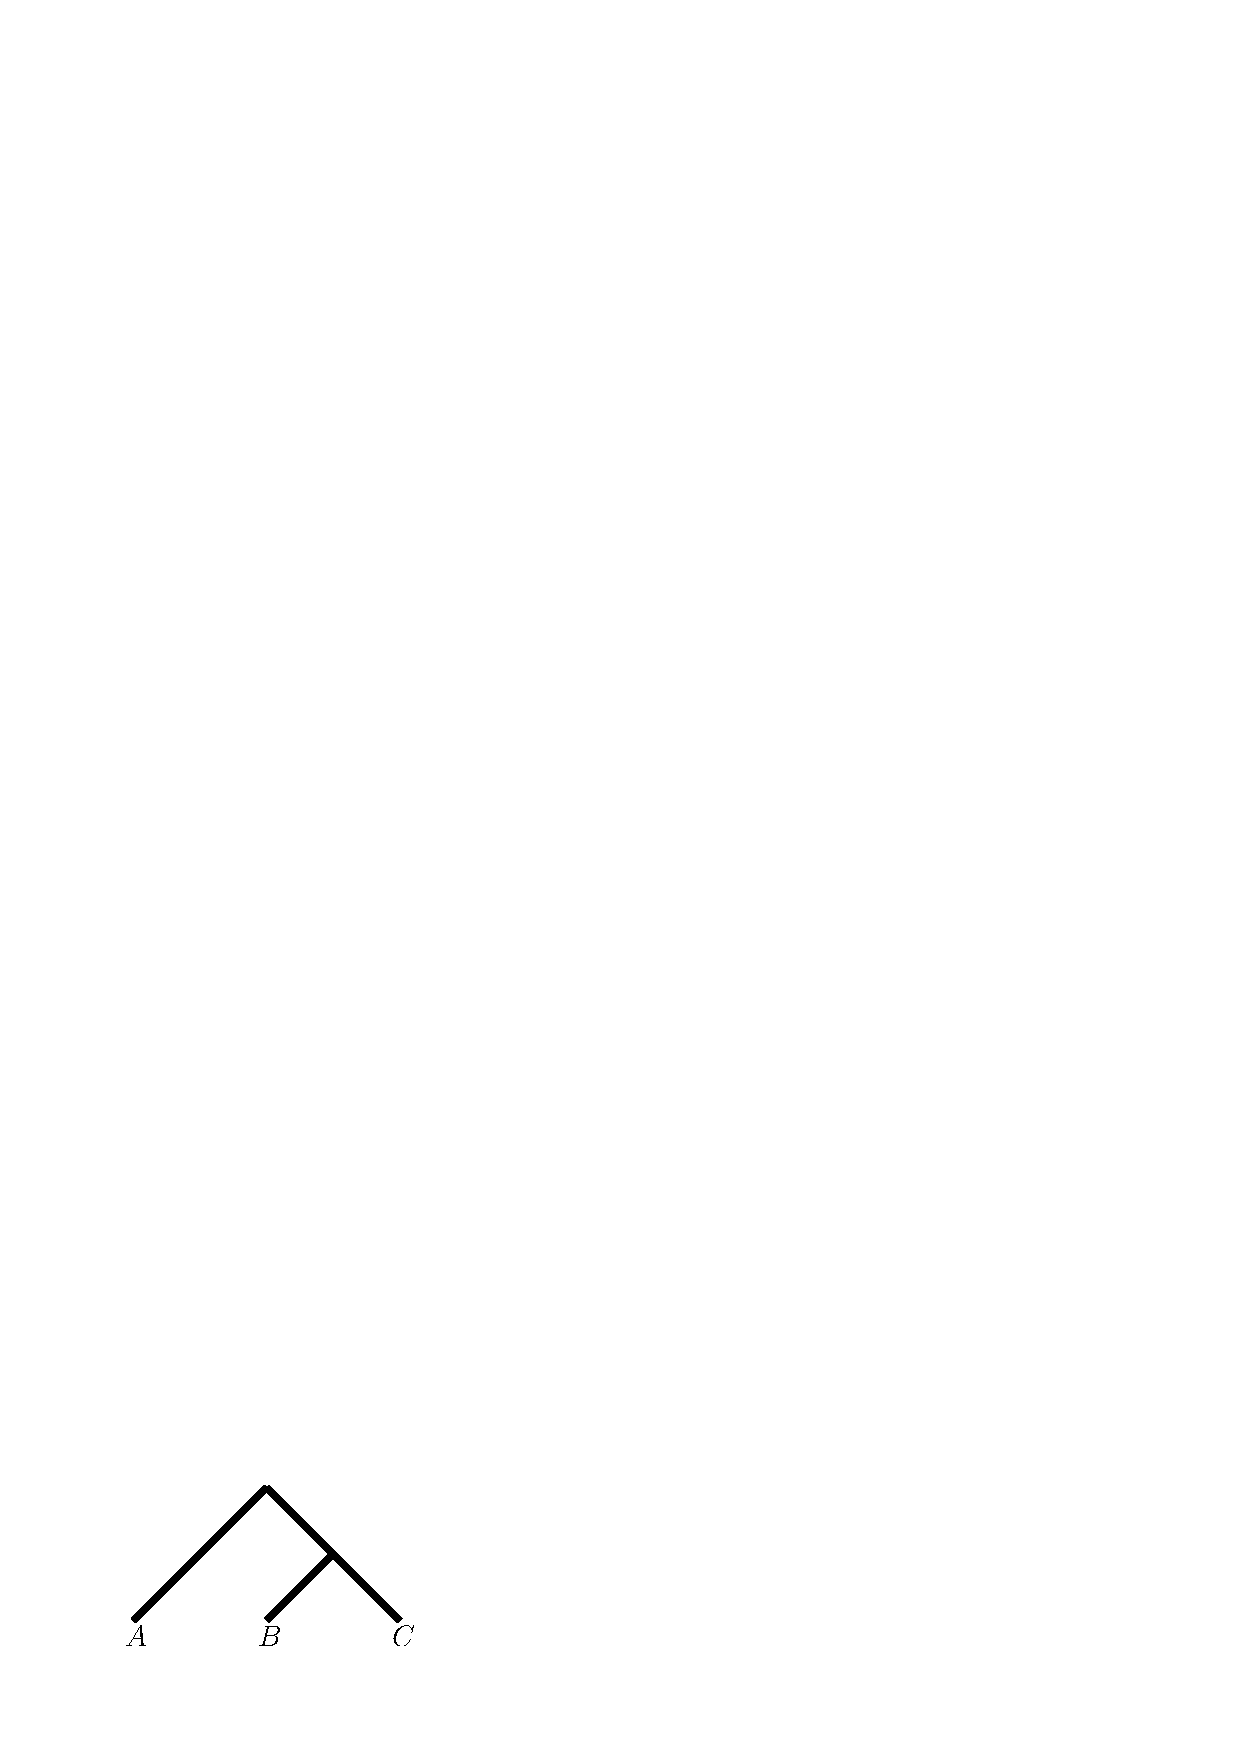
\includegraphics[width=0.6\linewidth]{Figs/TrueOne1.pdf}
            \end{center}
          \end{minipage}
          \\
          %% Replicate 3
	  & \\
	  \multicolumn{3}{c}{Bootstrap Replicate \#3}\\
	  $
          \begin{array}{|c|cccc|}
            \hline
            \textbf{A} & \gray{T} & \grey{T} & \grey{T} & \gray{T} \\
            \textbf{B} & \gray{A} & \grey{T} & \grey{T} & \gray{A} \\
            \textbf{C} & \gray{C} & \grey{C} & \grey{C} & \gray{C} \\
            \hline
          \end{array}
	  $
          &
          $\longrightarrow$
          &
          \begin{minipage}[c]{0.25\linewidth}
            \begin{center}
              
\includegraphics[width=0.6\linewidth]{Figs/TrueOne2.pdf}
            \end{center}
          \end{minipage}
          \\
	\end{tabular}
   \end{center}
   \caption{Principle of the bootstrap for phylogenies. Each character is identified by its color and style. Characters are sampled with replacement to produce bootstrap replicates, which are then used to infer phylogenies. The split $A|BC$ appears in $2$ out of $3$ bootstrap trees and therefore has a bootstrap value of $BP = 2/3$ or $66$\%.}
  \label{fig:bootstrap}
\end{figure}

Intuitively, the variation obtained by resampling $n$ sites from the original data should be the same as the variation obtained by sampling $n$ new characters. Bootstrap values capture, among other, the \emph{sampling} variability induced short MSA. When $n$ increases, so does $BP$ in general and it is quite common to achieve very high values for all branches when working on genome-scale alignments~\citep{Rokas2003}. 

$BP$ provides a guide for the amount of support a branch has: branches with high $BP$ occur more often and are more reliable than those with low $BP$. Although it might be tempting to interpret $BP$ as the probability that a branch is present in the (unknown) true tree, this is not the case in general. \cite{Zharkikh1992} showed in a simple case that $BP$ is biased and underestimates that probability. Using simulation studies, \cite{Hillis1993} showed that $BP$ values as small as 70\% could reflect highly supported branches. Many studies~\citep{Felsenstein1993, Efron1996, Susko2008, Susko2010} examined the theoretical properties of bootstrap values and concluded that they are indeed biased. This bias is partly induced by the peculiar geometry of tree space (see \cite{Billera2001, Susko2010} and Section~\ref{sec:extensions}). 

The final limitation of bootstrap values, shared with other support values based on resampling techniques, is that they are quite computationally expensive to compute: the computational budget required to compute $B$ bootstrap trees is roughly $B$-fold higher than the time required to compute the original tree, although clever tricks can reduce significantly~\citep{Stamatakis2006}.

%%%%%%%%%%%%%%%%%%%%%%%%%%%%
\subsubsection{Posterior Probabilities} \label{sec:posterior-probabilities}

Posterior Probabilities ($PP$) are mostly used in a Bayesian framework and similar in spirit bootstrap values. The main difference lies in the forest of trees used to compute support values. Bayesian procedures estimate the posterior distribution of trees. Due to the huge size of the tree space, Markov Chain Markov Chains (MCMC) are used in practice to produce a sample from this distribution~\citep{Yang1997a}. The $PP$ of a branch is computed, just like $BP$, as the the probability of occurence of that branch in the MCMC sample. MCMC trees constitute a set of highly likely trees (best, second best, etc) for the original dataset. $PP$ are easier to interpret than $BP$ as they approximate directly the probability that a branch is present in the true tree, given the original data. Furthermore, since MCMC trees are a natural byproduct of the estimation procedure, there is almost no overhead in computing $PP$. 

Unfortunately, $PP$ are not immune to bias. Empirical studies found that $PP$ are generally higher than $BP$~\citep{Anisimova2011} and sometimes even overconfident. The ``star-tree paradox'' \citep{Yang2007} is the most extreme example of spurrious support. \citet{Yang2007} showed that when the actual tree is a 3 species star-like, with no real inner branch, and that sequence length goes to $\infty$, one branch randomly chosen among the 3 potential but erroneous inner branches, has its $PP$ that goes to $100$\% whereas one would expect all potential branches to have $PP$ around $33$\%. 

Intuitively, $PP$ are higher than $BP$ because they cover fewer sources of variability. Unlike bootstrap trees, MCMC trees all originate from the same dataset. $PP$ are quite good at capturing the lack of phylogenetic signal in the original MSA but not the impact of a few influential characters. For example, outlier characters with a strong effect on tree inference will affect all MCMC trees consistently. By contrast, they will be included in some replciates but left out from others leading to more variation among bootstrap trees than among MCMC trees. Finally, in genome-scale context where inaccuracies are more likely to arise from modeling errors than from sampling variability, $PP$ are uniformly high and as uninformative as $BP$~\citep{Philippe2011, Kumar2012}

%%%%%%%%%%%%%%%%%%%%%%%%%%%%
\subsubsection{Others} \label{sec:other-confidence}

aLRT, SH, etc for each node

%%%%%%%%%%%%%%%%%%%%%%%%%%%%
\subsection{Outliers in the Data} \label{sec:outliers}

Note that bootstrap does not answer the question ``What is the probability that this branch is present in the actual phylogeny?''

%%%%%%%%%%%%%%%%%%%%%%%%%%%%
\subsubsection{Rogue Taxa} \label{sec:rogue-taxa}

%%%%%%%%%%%%%%%%%%%%%%%%%%%%
\subsubsection{Rogue Sites} \label{sec:rogue-sites}
